\documentclass[a4paper,11pt]{article}

\usepackage{préambule}
\usetikzlibrary{angles,quotes,intersections}

\mdfdefinestyle{rappelstyle}{
    style=greyboxstyle,
    frametitle={Rappel},
}
\newmdenv[style=rappelstyle]{rappel}

\title{Chapitre 6 : Angles, angles dans un triangles}
\date{}
\author{}

\begin{document}

\maketitle

\section*{Rappel sur les angles}

\begin{rappel}
	Si on a trois points $A$, $B$ et $C$, l'angle que forme les droites $(AB)$ et $(BC)$ est appelé $\widehat{ABC}$.

	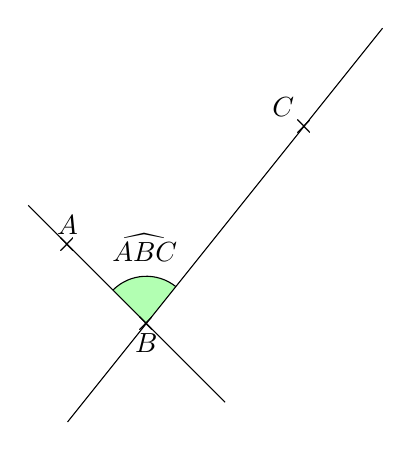
\begin{tikzpicture}
		\coordinate (A) at (-1,1);
		\coordinate (B) at (0,0);
		\coordinate (C) at (2,2.5);

		\draw pic[draw,fill=green!30,angle radius=0.6cm,"$\widehat{ABC}$" shift={(0mm,0.6cm)}] {angle=C--B--A};
		\draw (-1.5,1.5) -- (1,-1);
		\draw (-1,-1.25) -- (3,3.75);

		\node at (A) {×};
		\node at (B) {×};
		\node at (C) {×};
		\node[above] at (A) {$A$};
		\node[below] at (B) {$B$};
		\node[above left] at (C) {$C$};
	\end{tikzpicture}
\end{rappel}

\begin{rappel}
	Si on a deux droite $(d₁)$ et $(d₂)$ qui s'intersectent en $D$, l'angle que forment ces deux droite est appelé $d₁Dd₂$.

	\begin{tikzpicture}
		\coordinate (A) at (-1,1);
		\coordinate (B) at (0,0);
		\coordinate (C) at (3,1.5);

		\draw pic[draw,fill=blue!30,angle radius=0.6cm,"$\widehat{ABC}$" shift={(0mm,0.6cm)}] {angle=C--B--A};
		\draw (-1.5,1.5) node[above] {$d₁$} -- (1,-1);
		\draw (-2,-1) node[above] {$d₂$} -- (C);

		\node at (B) {×};
		\node[below] at (B) {$D$};
	\end{tikzpicture}
\end{rappel}

\section{Angles alternes-internes}

% TODO: trouver une meilleure explication.
\begin{cours}[Angles alternes-internes]
	Soit $(d)$ et $(d')$ des droites, et $(s)$ une droite qui intersecte $(d)$ et $(d')$ en $A$ et $B$.

	Alors, deux angles sont \textbf{alternes-internes} si:
	\begin{itemize}
		\item Ils ont pour sommet $A$ et $B$.
		\item Ils sont chacun d'un côté différent de la droite $(s)$.
		\item Ils sont entre les droites $(d)$ et $(d')$.
	\end{itemize}

	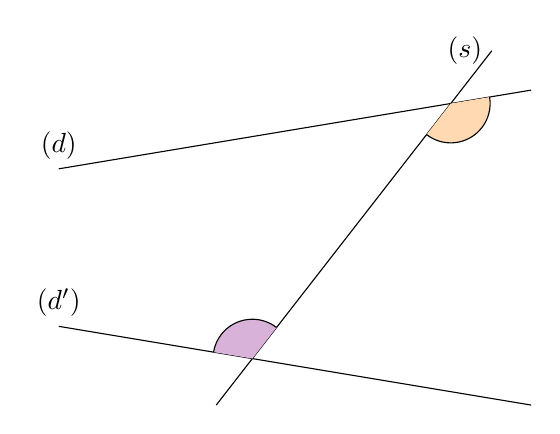
\begin{tikzpicture}
		\coordinate (dprimestart) at (-2,-1);

		\draw[name path=d] (-2,1) node[above] (dstart) {$(d)$} -- (4,2) coordinate (dend);
		\draw[name path=dprime] (dprimestart) node [above] {$(d')$} -- (4,-2) coordinate (dprimeend);
		\draw[name path=s] (3.5,2.5) node[left] {$(s)$} -- (0,-2);

		\path[name intersections={of= d and s,by=A}];
		\path[name intersections={of= dprime and s,by=B}];

		\draw pic[draw,fill=orange!30,angle radius=0.5cm] {angle=B--A--dend};
		\draw pic[draw,fill=violet!30,angle radius=0.5cm] {angle=A--B--dprimestart};
	\end{tikzpicture}
\end{cours}

\begin{exemple}
	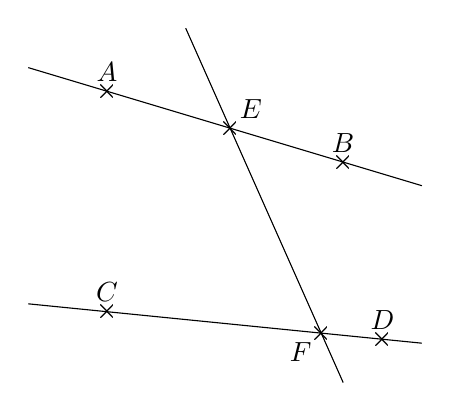
\begin{tikzpicture}
		\coordinate (d1-1) at (-2,3);
		\coordinate (d1-2) at (-1,2.7);
		\coordinate (d1-3) at (2,1.8);
		\coordinate (d1-4) at (3,1.5);

		\draw[name path=d-1] (d1-1) -- (d1-4);
		\node at (d1-2) {×};
		\node[above] at (d1-2) {$A$};
		\node at (d1-3) {×};
		\node[above] at (d1-3) {$B$};

		\coordinate (d2-1) at (-2,0);
		\coordinate (d2-2) at (-1,-0.1);
		\coordinate (d2-3) at (2.5,-0.45);
		\coordinate (d2-4) at (3,-0.5);

		\draw[name path=d-2] (d2-1) -- (d2-4);
		\node at (d2-2) {×};
		\node[above] at (d2-2) {$C$};
		\node at (d2-3) {×};
		\node[above] at (d2-3) {$D$};

		\draw[name path=s] (0,3.5) -- (2,-1);

		\path[name intersections={of= d-1 and s,by=E}];
		\path[name intersections={of= d-2 and s,by=F}];

		\node at (E) {×};
		\node[above right] at (E) {$E$};
		\node at (F) {×};
		\node[below left] at (F) {$F$};
	\end{tikzpicture}

	Sur cette figure, les angles
	\begin{itemize}
		\item $\widehat{FEA}$ et $\widehat{EFD}$ sont alternes-internes.
		\item $\widehat{BEF}$ et $\widehat{CFE}$ sont alternes-internes.
	\end{itemize}
\end{exemple}


\end{document}